\chapter{Systembeskrivelse}
Dette kapitel indeholder en introducerende beskrivelse af den udviklede prototype, herunder brugergrænsefladen og fysisk opbygning.

Figur \ref{fig:system} viser den overordnede opbygning af systemet. Grundlæggende består systemet af en beholder indeholdene opløsningen med langerhanske øer. Opløsningen pumpes herefter ved hjælp af en pumpe i gennem en slange, hvor et kamera detektere om en ø passere eller ej. Hvis en ø er detekteret åbner systemet en ventil for at frasortere øen fra resten af opløsningen. Systemet består af et software program udviklet i Matlab, hvor operatøren har mulighed for at interagere med systemet. Her er selve logikken og signalbehandlingen i form af billedprocessering implementeret. Programmet giver signal til en Microcontroller (Arduino platform), som håndterer styring af hardware komponenterne.

\begin{figure}[H]
	\centering
	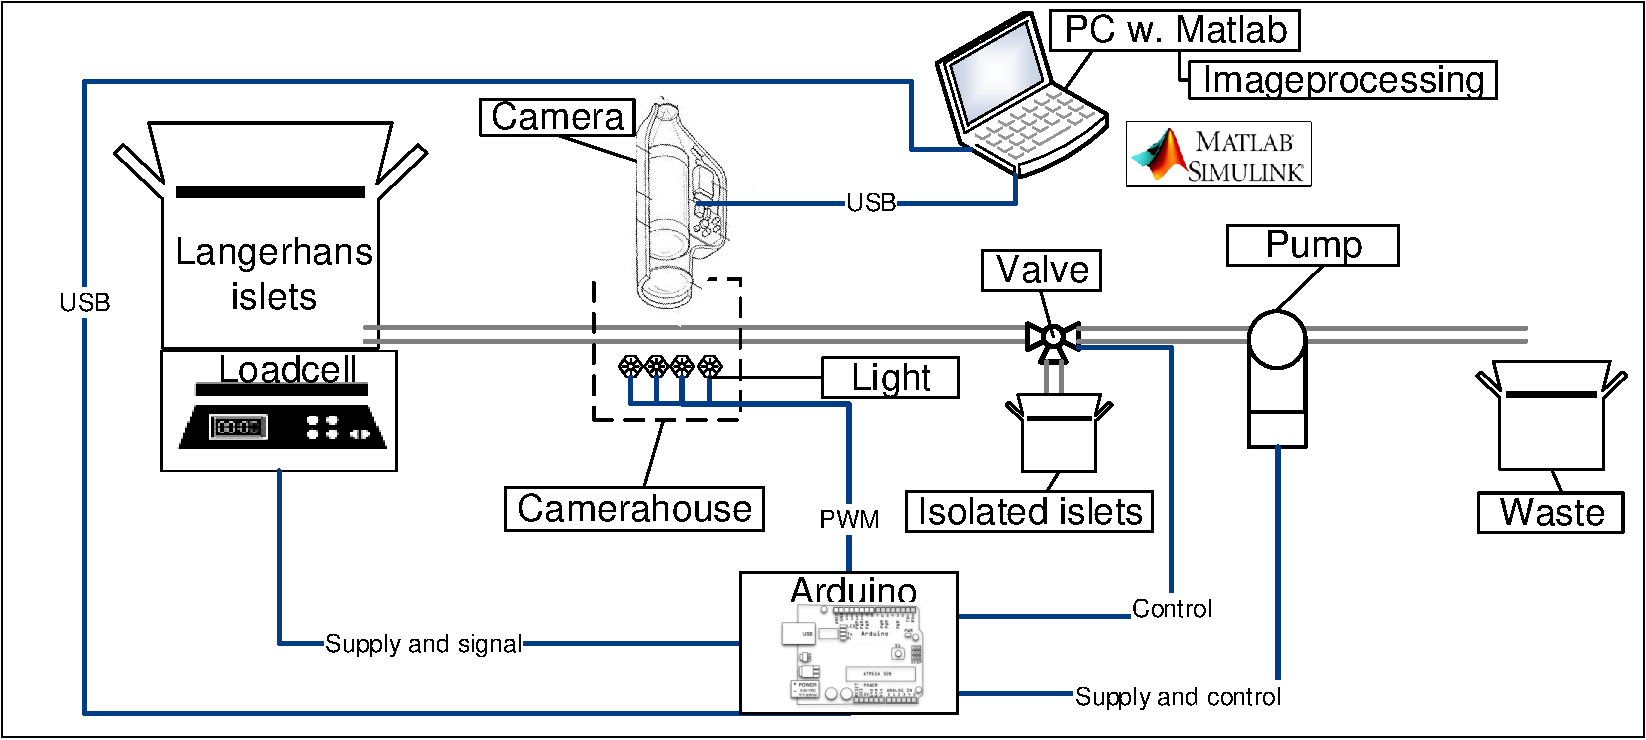
\includegraphics[width=1\textwidth]{billeder/DMTS.pdf}
	\caption{Figuren viser den overordnede opbygning af systemet}
	\label{fig:system}
\end{figure}
Beskrivelse 

Figur over systemet

Billeder af det færdige system

\section{Brugergrænseflade}
Billeder og beskrivelser


